\documentclass[../MasterThesis.tex]{subfiles}
\graphicspath{ {./assets/images/} }


%----------------------------------------------------------------------------
%----------------------------------------------------------------------------

\begin{document}
	

%
%
%
%
%=======================================================================================================
%
%
%
%
%=======================================================================================================
% CHAPTER: Preliminaries
%=======================================================================================================
\newpage
% \section{Preliminaries} \label{section:preliminaries}

\section{Theoretical Foundation of Colour} \label{section:theoreticalfoundationofcolour}

In this Chapter, the terms colour correction and colour grading are introduced and the effects of different colours in media and their association are explained. Additionally, the RGB colour model is presented and a method for the comparison of different colour saturations using GIMP is shown.





%-------------------------------------------------------------------------------------------------------
\subsection{Colour Correction and Colour Grading} 


Colour correction and colour grading are both processes used in film making, photography and digital art to adjust and enhance the colour of images or videos. 
While they are related, they serve different purposes and are typically performed at different stages of production.

Colour correction aims to correct technical imperfections and achieve a natural-looking image, while colour grading focuses on enhancing the visual aesthetics and storytelling aspects.~\cite{cc_cg_1, cc_cg_2}


Colour correction is the process of adjusting the overall colour balance, contrast and exposure of an image or video to achieve a more accurate representation of the scene as it was captured by the camera. It involves correcting potential technical issues such as white balance, exposure inconsistencies and colour inaccuracies caused by the camera or lighting conditions.
This is typically done in the early stages of post-production to ensure that the footage looks natural and consistent across different shots and scenes.~\cite{cc1, cc_cg_1, cc_cg_2}


Colour grading, on the other hand, is the creative process of altering the colour and mood of an image or video to evoke a specific aesthetic or emotional response. The effects of different colours are described in Section~\ref{subsection:effectsofdifferentcolours}.
Colour grading involves making stylistic choices to enhance the visual storytelling or the overall cinematic look or perception of the footage. It can involve manipulating individual colours, adjusting contrast, saturation and various other image manipulation techniques. Colour grading is often performed after colour correction and is considered a more artistic and subjective process. It allows film makers and photographers to establish a unique visual style and enhance the narrative impact of their work.~\cite{cc_cg_1, cc_cg_2}


In summary, colour correction and colour grading serve different purposes and are performed at different stages of post-production. Colour correction ensures technical accuracy and consistency, while colour grading adds artistic components and enhances the visual storytelling and perception of the footage.~\cite{cc1, cc_cg_1, cc_cg_2}








%-------------------------------------------------------------------------------------------------------
% \subsection{Colour Theory}










\newpage
%-------------------------------------------------------------------------------------------------------
\subsection{Effects of Different Colours} 
\label{subsection:effectsofdifferentcolours}

Different colours can convey a different understanding of a scene to the viewer or even influence the viewers emotions. 
Different colours have distinct psychological associations, which influence how viewers perceive and interpret the content.~\cite{colour,colour2}
%But it needs to be considered that colours can carry cultural and contextual meanings that can vary across different societies and individuals. 


In different visual media, including photos and videos, the strategic use of colour can effectively communicate themes, evoke emotions and guide viewer interpretation.~\cite{cc_cg_1, cc_cg_2, colour, colour2}


In the following, different colours with their psychological associations are listed and example pictures are shown.



%-------------------------------------------------------------------------
%\subsubsection{Red}
\textbf{\textcolor{Maroon}{Red}}

%
%

\begin{minipage}{0.5\textwidth}
	\begin{figure}[H]
		\begin{center}
			\cutpic{0.3cm}{\textwidth}{fliegenpilz.jpg}
			\caption[Picture of a Amanita muscaria in Sweden with alarming red colour.]{Picture of a Amanita muscaria in Sweden with alarming red colour.}
			\label{figure:red}
		\end{center}
	\end{figure}
 \hfill
\end{minipage}\begin{minipage}{0.05\textwidth}
	\ 
\end{minipage}\begin{minipage}{0.45\textwidth}
	The colour red is often associated with intense emotions such as passion, excitement and danger. Viewing it on self or others has even been shown to increase the perception of aggressiveness and dominance.~\cite{red_dominance} Wearing the colour in sport competitions and events, red has been shown to enhance performance and the perceived performance.~\cite{colour, red_sport}
	
	In visual media, the use of red can evoke feelings of urgency, power and love. For example a video with flashes of red light may create a feeling of tension or alarm while a female wearing red can increase the perceived attraction.~\cite{colour, red_romance}
	
	Beyond its symbolism in human emotions and cultural contexts, red also serves as a prominent warning colour in nature. One example of this is the
	
\end{minipage}

\vspace*{-0.6em}
toxic fly agaric mushroom (Amanita muscaria), which can be seen in Figure~\ref{figure:red}.
The instinctual reaction to red is used in various contexts, including traffic signals and emergency exits, where the color serves as a clear and universally understood signal.







\newpage
%-------------------------------------------------------------------------
%\subsection{Blue} 
\textbf{\textcolor{BlueViolet}{Blue}}

%
\begin{minipage}{0.45\textwidth}
	The colour blue is often linked to feelings of calmness and stability. In videos and pictures, the presence of blue tones can create a sense of relaxation. For instance, the photo in Figure~\ref{figure:blue} of a lake scene in Sweden with shades of blue in the water and the sky can evoke a peaceful mood.
	
	Additionally, blue stores and logos have been shown to increase the perception of expected quality and trustworthiness.~\cite{blue_trust, colour2}
	
	But this is not the only association with the colour blue. While it might
	
	
	
\end{minipage}\begin{minipage}{0.05\textwidth}
	\ 
\end{minipage}\begin{minipage}{0.5\textwidth}
	\begin{figure}[H]
		\begin{center}
			\cutpic{0.3cm}{\textwidth}{lake.jpg}
			\caption[Picture of a lake in Sweden with mainly blue tones.]{Picture of a lake in Sweden with mainly blue tones.}
			\label{figure:blue}
		\end{center}
	\end{figure}\hfill
\end{minipage}

\vspace*{-0.6em}
evoke feelings of calmness or trustworthiness in certain contexts, it can also represent sadness or coldness depending on the situation.~\cite{colour2}


%-------------------------------------------------------------------------
%\subsection{Green}
\textbf{\textcolor{ForestGreen}{Green}}

%
%
\begin{minipage}{0.5\textwidth}
	\begin{figure}[H]
		\begin{center}
			\cutpic{0.3cm}{\textwidth}{forest.jpg}
			\caption[Picture of a forest in Sweden with mainly green tones.]{Picture of a forest in Sweden with mainly green tones.}
			\label{figure:green}
		\end{center}
	\end{figure}\hfill
\end{minipage}\begin{minipage}{0.05\textwidth}
	\ 
\end{minipage}\begin{minipage}{0.45\textwidth}
	Green is associated with nature, growth and harmony. In visual media, the use of green can symbolize renewal, freshness and balance. Green is a colour that appears often in nature, because it is the result of chlorophyll, a substance in plants that helps them to turn sunlight into energy.~\cite{green, colour2}
	
	For example, the picture in Figure~\ref{figure:green} of a forest in Sweden can evoke feelings of vitality  and  may convey a sense of natural beauty and harmony, because the plants in this picture show a lot of green tones.~\cite{greenwashing}
	

	
	
\end{minipage}

	\vspace*{-0.6em}

	Additionally, green is often used in environmental campaigns and eco-friendly branding to signify sustainability and a connection to the earth. 








\newpage
%-------------------------------------------------------------------------
%\subsection{Yellow}
\textbf{\textcolor{YellowOrange}{Yellow}}


%
\begin{minipage}{0.45\textwidth}
	Yellow is often associated with happiness, optimism and energy. When used in videos or pictures, yellow can evoke feelings of warmth, cheerfulness and positivity. For instance, a photograph capturing a bright yellow sunrise as seen in Figure~\ref{figure:yellow} can convey a sense of warmth, hope and optimism.
	
	In media editing, the colour yellow can be increased to convey the impression of sunshine or a sunny day to the viewer.
	
	Moreover, yellow is used in the realm of marketing and advertising. Brands often apply the colour yellow to evoke 
	
	
\end{minipage}\begin{minipage}{0.05\textwidth}
	\ 
\end{minipage}\begin{minipage}{0.5\textwidth}
	\begin{figure}[H]
		\begin{center}
			\cutpic{0.3cm}{\textwidth}{sunset.jpg}
			\caption[Picture of a sunrise in Sweden with mainly yellow tones.]{Picture of a sunrise in Sweden with mainly yellow tones.}
			\label{figure:yellow}
		\end{center}
	\end{figure}\hfill
\end{minipage}

% \vspace*{-0.6em}
positive associations with their products, because of its cheerful and optimistic connotations. It also plays a role in interior design: A room painted in soft yellow tones can convey feelings of warmth, making it an ideal choice for homes.~\cite{colour2}




%-------------------------------------------------------------------------
%\subsection{Black and White}

\textbf{\textcolor{gray}{Black and white}}


\begin{minipage}{0.5\textwidth}
	\begin{figure}[H]
	\begin{center}
		\cutpic{0.3cm}{\textwidth}{dubai2.jpg}
		\caption[Picture of skyscrapers in Dubai in greyscales.]{Picture of skyscrapers in Dubai in greyscales.}
		\label{figure:gray}
	\end{center}
\end{figure}\hfill
\end{minipage}\begin{minipage}{0.05\textwidth}
	\ 
\end{minipage}\begin{minipage}{0.45\textwidth}
	Black and white or greyscales are often used to evoke a sense of timelessness or simplicity. In visual media, the absence of colour can draw attention to shapes, textures and contrasts. For example, a black and white photograph of a city skyline can emphasize the architectural details and create a dramatic atmosphere or, depending on the context, it may evoke a sense of nostalgia.
	In Figure~\ref{figure:gray}, houses in Dubai can be seen. The greyscale filter of this photo enhances the focus of the viewer on the architecture and the structures

	
\end{minipage}

\vspace*{-0.6em}
 of the buildings. Furthermore, black, white and greyscale are often used to convey elegance and simplicity.~\cite{colour2}


%





%-----------------------------------------------------------------------------------
\subsection{RGB Colour Representation}
\label{subsection:RGB}


RGB colour representation is a method to display colours on screens. It stands for Red, Green and Blue. 
Each of those colour channels (red, green and blue) has a value ranging from 0 to 255. When all three colours are at their maximum value with \texttt{(255,255,255)}, the outcome is white. On the contrary, when all three colour channels are at their minimum value with \texttt{(0,0,0}), the result is black.~\cite{colourRGB}

The three colours are combined in with different values to create the broad spectrum of colours. The red, green and blue values use 8 bits each. This results into $16\ 777\ 216$ possible colours.



For example the colour red can be created with mixing full red (255 in the red channel), no green (0 in the green channel) and no blue (0 in the blue channel). This leads to a pure red as \texttt{(255,0,0)}.
This red can be adjusted by varying the values in the other colour channels. By decreasing the red value, tones such as a dark maroon with \texttt{(130,0,0)} can be achieved and with a higher red and green value a vibrant crimson with \texttt{(200,50,10)} can be achieved. On the other hand, by increasing blue while maintaining a high red channel, tones including scarlet \texttt{(255,40,0)} or coral \texttt{(255,120,80)} can be created. In addition to this, introducing equal amounts of green and blue alongside the high red value can transition the colour into a softer tone, such as rose \texttt{(255,150,150)}. The described colours can be seen in Figure~\ref{figure:RGBred}.




\begin{figure}[H]
	\centering
	
	\begin{tabular}{cccccc}
		
		
		\textcolor[RGB]{130,0,0}{\rule{2cm}{2cm}} &
		\textcolor[RGB]{200,50,10}{\rule{2cm}{2cm}} &
		\textcolor[RGB]{255,0,0}{\rule{2cm}{2cm}} &
		\textcolor[RGB]{255,40,0}{\rule{2cm}{2cm}} &
		\textcolor[RGB]{255,120,80}{\rule{2cm}{2cm}} &
		\textcolor[RGB]{255,150,150}{\rule{2cm}{2cm}} \\
		
	
		\scriptsize{\centering \texttt{(130,0,0)}} &
		\scriptsize{\centering \texttt{(200,50,10)}} &
		\scriptsize{\centering \texttt{(255,0,0)}} &
		\scriptsize{\centering \texttt{(255,40,0)}} &
		\scriptsize{\centering \texttt{(255,120,80)}} &
		\scriptsize{\centering \texttt{(255,150,150)}} \\
		
		
		
	\end{tabular}
	
	
	\caption[Different shades of red represented by different RGB values.]{Different shades of red represented by different RGB values.}
	\label{figure:RGBred}
	
\end{figure}



Each pixel on a display consists of three sub-pixels that each display one of the colours red, green and blue. By adjusting the intensity of each sub-pixel, a wide range of colours can be achieved. 
The RGB value of a pixel indicates the amount of each colour. This means if for example the red pixel is set to 0, the red LED is turned off. When the red pixel is set to 255, the red LED is turned fully on.~\cite{colourRGB}

The RGB colour model is an additive colour model, which is the opposite to subtractive colour models that apply to paints and other substances where the colour reflects certain components of the light. 
In the subtractive model, a paint filters out all colours but its own and two blended colours filter out all colours but the common colour between them. In the additive model, the colour has a brightness that is the sum of the brightness of the two mixed colours. Because of this, mixed colours appear brighter than individual colours.~\cite{colourRGB}

A colour diagram that shows the additive model of RGB can be seen in Figure~\ref{figure:RGB} and the subtractive model can be seen in Figure~\ref{figure:othercolourwheel}.


\begin{minipage}{0.48\textwidth}
	\begin{figure}[H]
		
		\centering
		
		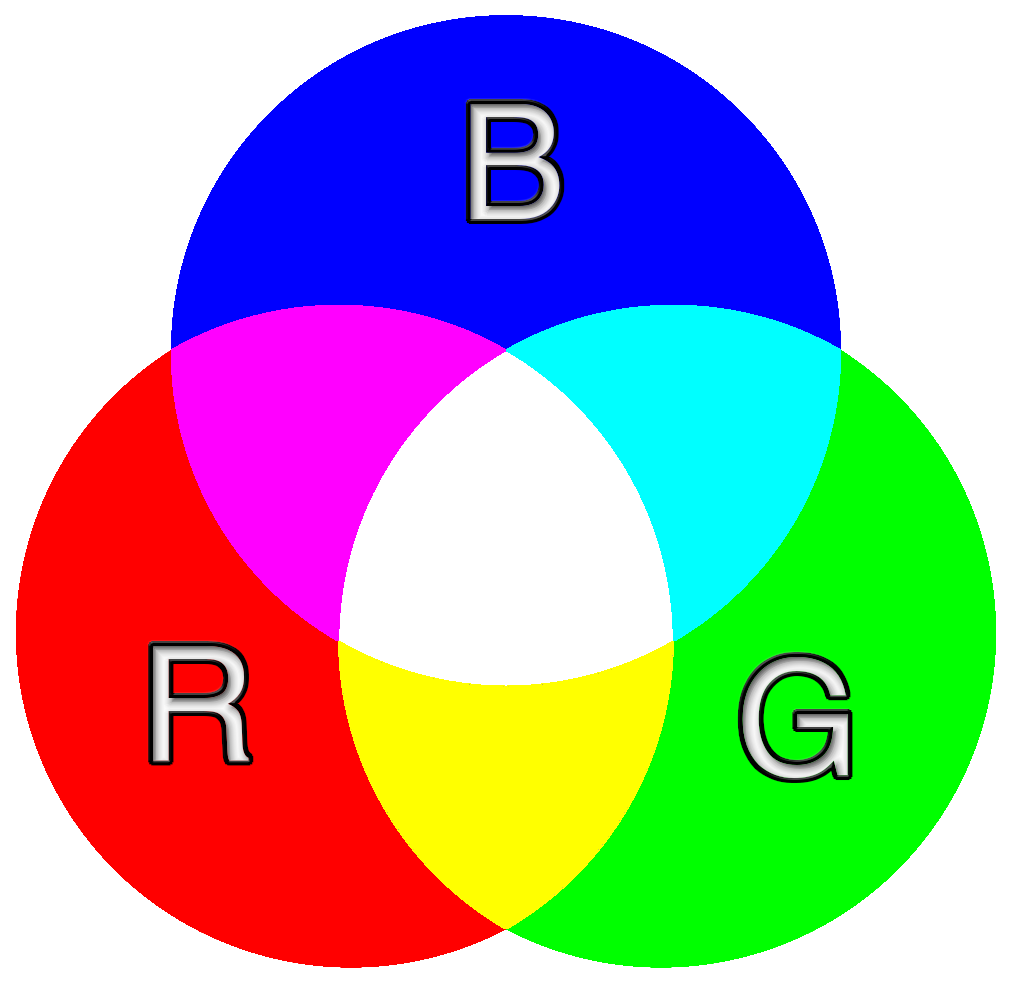
\includegraphics[width=0.8\textwidth]{RGB.png}
		
		\caption[Additive colour model of RGB]{Three coloured circles in red, green and blue showing the function of the additive colour model of RGB.}
		\label{figure:RGB}
		
	\end{figure}
\end{minipage}\begin{minipage}{0.04\textwidth}
\ 
\end{minipage}\begin{minipage}{0.48\textwidth}
\begin{figure}[H]
	
	\centering
	
	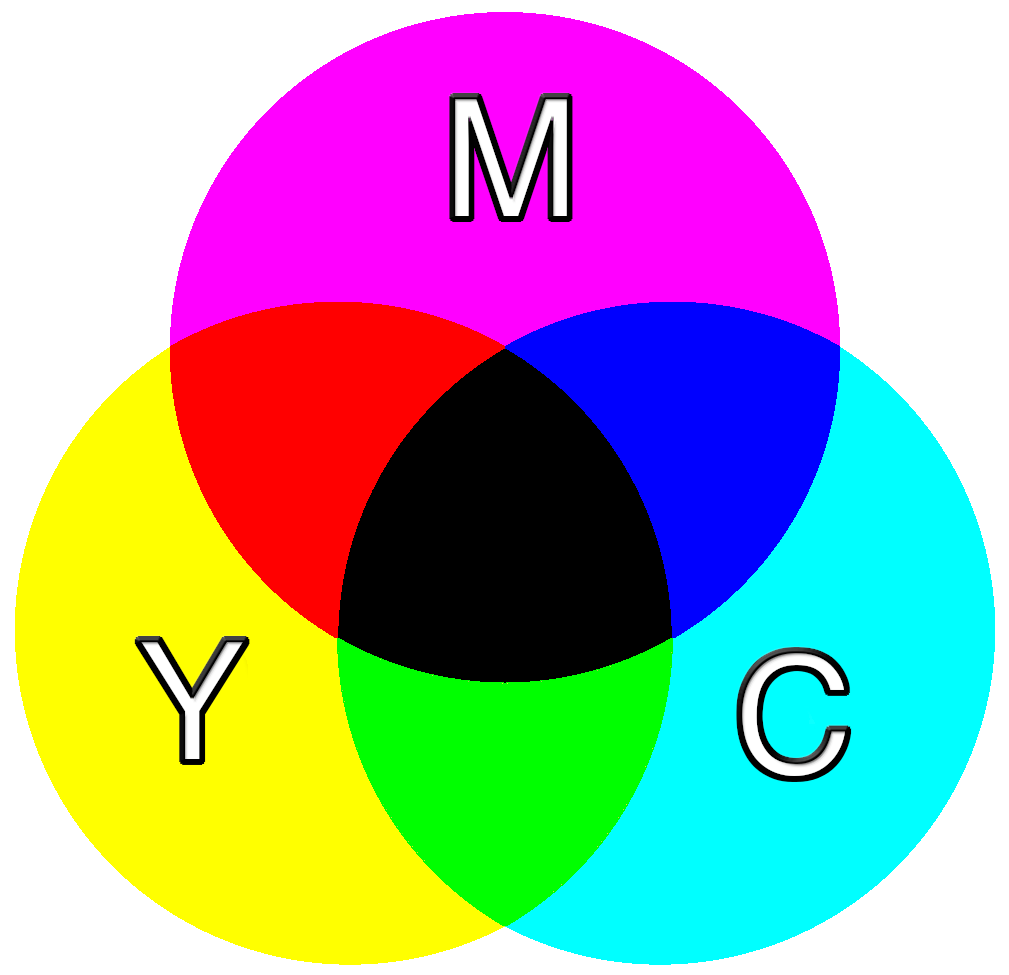
\includegraphics[width=0.8\textwidth]{YMCA.png}
	
	\caption[Subtractive colour model of RGB]{Three coloured circles in magenta, yellow and cyan showing the function of the subtractive colour model.}
	\label{figure:othercolourwheel}
	
\end{figure}
\end{minipage}

\vspace*{1em}



% Poynton, Charles A. "Digital Video and HDTV: Algorithms and Interfaces." Morgan Kaufmann Publishers, 2012.






%-----------------------------------------------------------------------------------
\subsection{Comparison of Different Colour Saturations with GIMP}
\label{subsection:ComparisonOfDifferentColourSaturations}



In this Section, a method for analysing the differences between two images is explained, where the colours of the images are subtracted from each other by using the image manipulation program GIMP. 
This method in GIMP is called \textit{grain extract} and it subtracts the colour values of corresponding pixels from two images to show any differences. It is a visual representation of the colour subtraction process, where subtracting identical pixels from each other results in a grey image, indicating no differences.~\cite{gimp}


When subtracting one image from another, the pixel values from one image are subtracted from the corresponding pixel values in the other image. 
The result reflects the relative differences in the colour values between the two subtracted images. For example with the subtraction of two red toned images, areas where the subtracted image has a less intense red tone will result into red pixels after the subtraction and analogical, areas where the subtracted image has a more intense red tone will result into green or blue pixels in the result of the subtraction. The result of the subtracted pixels depends on the difference between the two colour values.

Two examples of the colour subtraction with different red values can be seen in Figure~\ref{figure:neonminuslight}. In the Figure, the red colours \texttt{RGB(202, 95, 95)} and \texttt{RGB(255,0,0)} are subtracted from each other with the \textit{grain extract} function. This results in a blue colour (\texttt{RGB(74, 223, 223)}) and a different red tone (\texttt{RGB(181, 33, 33)}). 


% RGB:
% neon= 255, 0,0
% light= 202, 95, 95
% outcome blue = 74, 233, 233
% outcome red= 180, 32, 32




\begin{figure}[H]
	
	\centering
	
	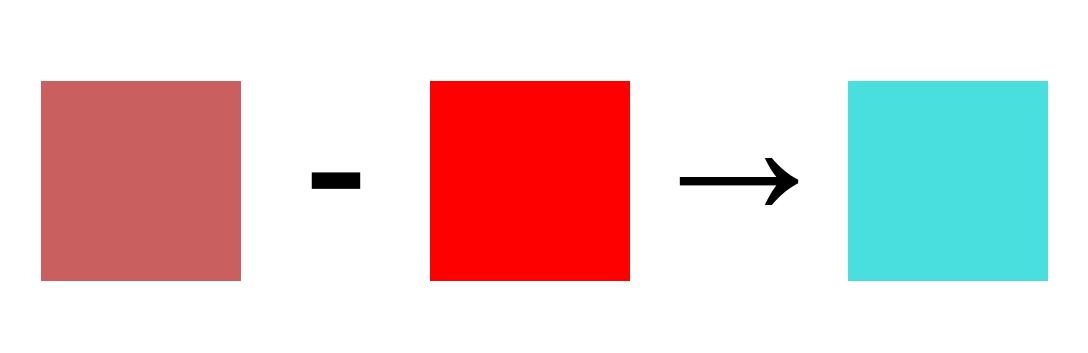
\includegraphics[width=0.6\textwidth]{lightMINUSneon.png}
	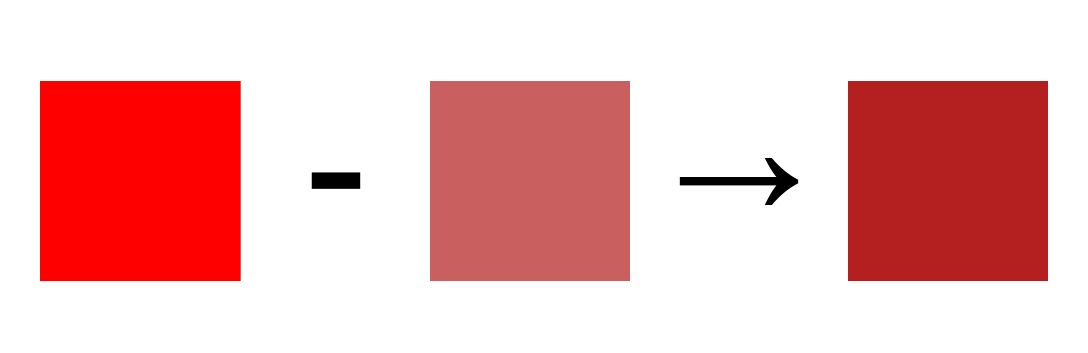
\includegraphics[width=0.6\textwidth]{neonMINUSlight.png}
	
	\caption[Colour subtraction with the GIMP function \textit{grain extract}.]{Subtraction of two different red values from each other with the GIMP function \textit{grain extract} to visualize the differences.}
	\label{figure:neonminuslight}
	
\end{figure}

The calculation to retrieve the new RGB values is defined and explained in the following.
Let $g$ be the \textit{grain extract} function in GIMP that adds 128 to two subtracted RGB values. The function is defined as follows:
%
\begin{align*}
	g(x, y) = x - y + 128
\end{align*}

Let $\text{\texttt{RGB}}_1$ and $\text{\texttt{RGB}}_2$ be the RGB values of a pixel in the same position in two different images, that are being subtracted.
%
\begin{align*}
	\text{\texttt{RGB}}_1 = (R_1, G_1, B_1) \ \ \ \ \ \ \ \ \ \ \ \ \ 
	\text{\texttt{RGB}}_2 = (R_2, G_2, B_2)
\end{align*}

The function $g$ can be applied to the RGB value pairs to retrieve the new values of the colours after the subtraction.
%
\begin{align*}
	\text{\texttt{RGB}}_1 - \text{\texttt{RGB}}_2 & \Rightarrow (g(R_1, R_2), g(G_1, G_2), g(B_1, B_2)) \\
	 & \Leftrightarrow ((R_1 - R_2 + 128), (G_1 - G_2 + 128) , (B_1 - B_2 + 128)) 
\end{align*}


For the examples, that are shown in Figure~\ref{figure:neonminuslight}, the calculations are shown in the following, with the RGB values $\text{\texttt{RGB}}_1 = (202, 95, 95)$ and
$\text{\texttt{RGB}}_2 = (255, 0, 0)$.
%
\begin{align*}
	\text{\texttt{RGB}}_1 - \text{\texttt{RGB}}_2 & \Rightarrow (g(202, 255), g(95, 0), g(95, 0)) \\
	 & \Leftrightarrow ((202 - 255 + 128), (95 - 0 + 128) , (95 - 0 + 128)) \\
	 & \Leftrightarrow (75, 223, 223) 
\end{align*}
%
%
\begin{align*}
	\text{\texttt{RGB}}_2 - \text{\texttt{RGB}}_1 & \Rightarrow (g(255, 202), g(0, 95), g(0, 95)) \\
	 & \Leftrightarrow ((255 - 202 + 128), (0 - 95 + 128) , (0 - 95 + 128)) \\
	 & \Leftrightarrow (181, 33, 33) 
\end{align*}

The results are the light blue colour \texttt{RGB(74, 223, 223)} and the red tone \texttt{RGB(181, 33, 33)}, that can be seen in Figure~\ref{figure:neonminuslight}. 


% RGB:
% neon= 255, 0,0
% light= 202, 95, 95
% outcome blue = 74, 233, 233
% outcome red= 180, 32, 32


















	
	
	
	
\end{document}